\section{U-Net Appendix}\label{s:unetAppendix}

\begin{figure}[H]
  \begin{center}
    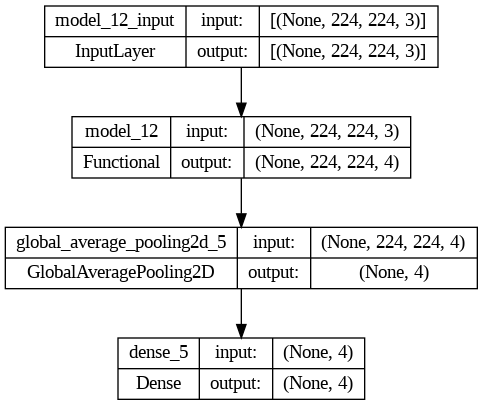
\includegraphics[width=0.35\textwidth]{unet/unetpp_model2.png}
  \end{center}
  \caption{U-Net++ model architecture}\label{fig:unetpp_model}
\end{figure}

Where \texttt{model\_12} is the U-Net++ model with EfficientNetB1 encoder. The Output Layer of \texttt{model\_12} is also used for the segmentation attempt to show what the model deems as the important parts of the image for the classification task.

\subsection{Additional Segmentation Results}

\begin{figure}[H]
  \centering
  \begin{subfigure}[b]{0.23\textwidth}
    \centering
    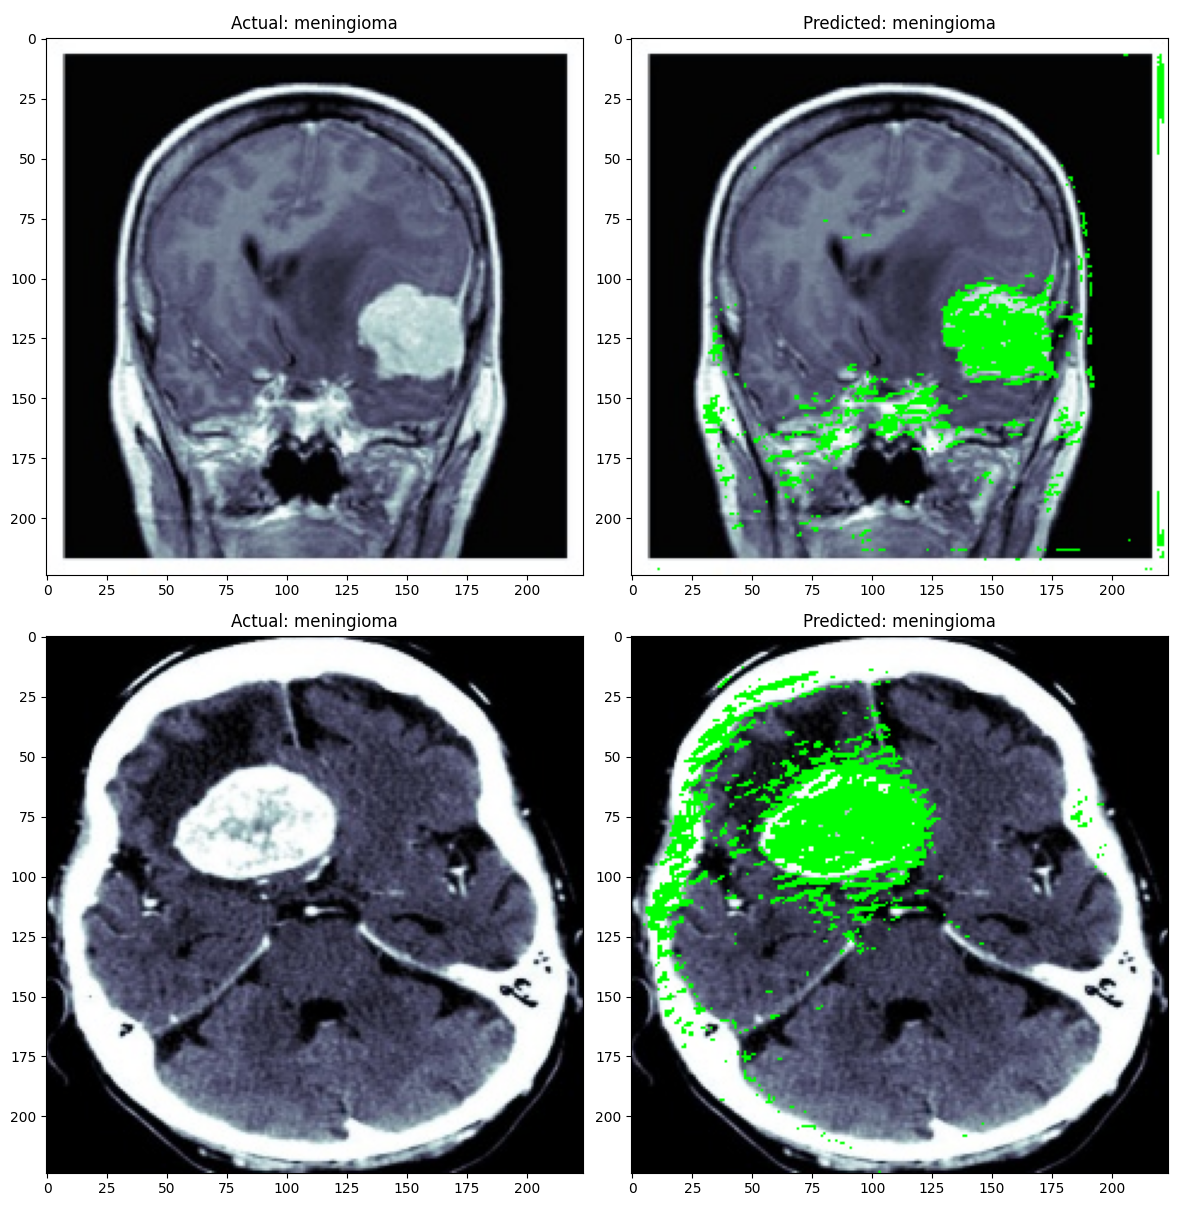
\includegraphics[width=\textwidth]{unet/evaluation/meningioma_1.png}
  \end{subfigure}
  \hfill
  \begin{subfigure}[b]{0.23\textwidth}
    \centering
    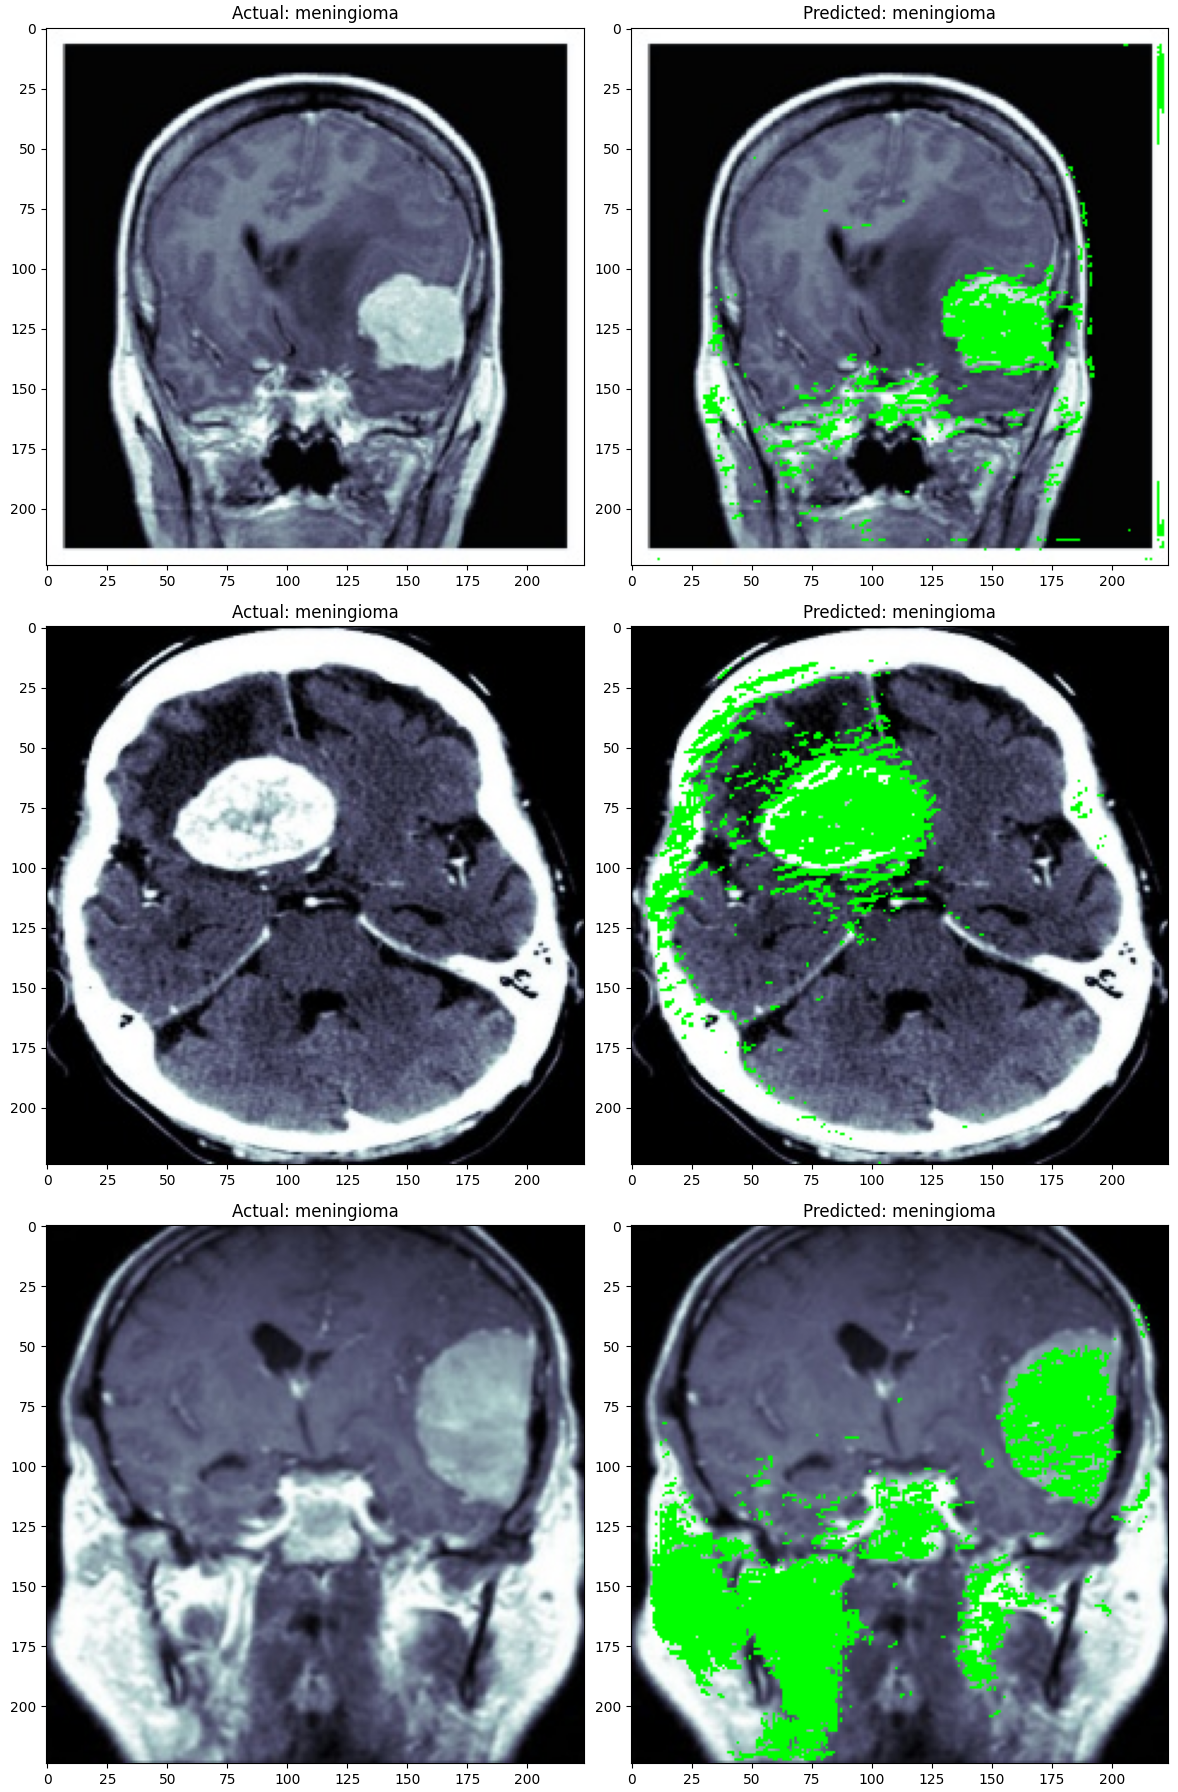
\includegraphics[width=\textwidth]{unet/evaluation/meningioma_2.png}
  \end{subfigure}
  \hfill
  \begin{subfigure}[b]{0.23\textwidth}
    \centering
    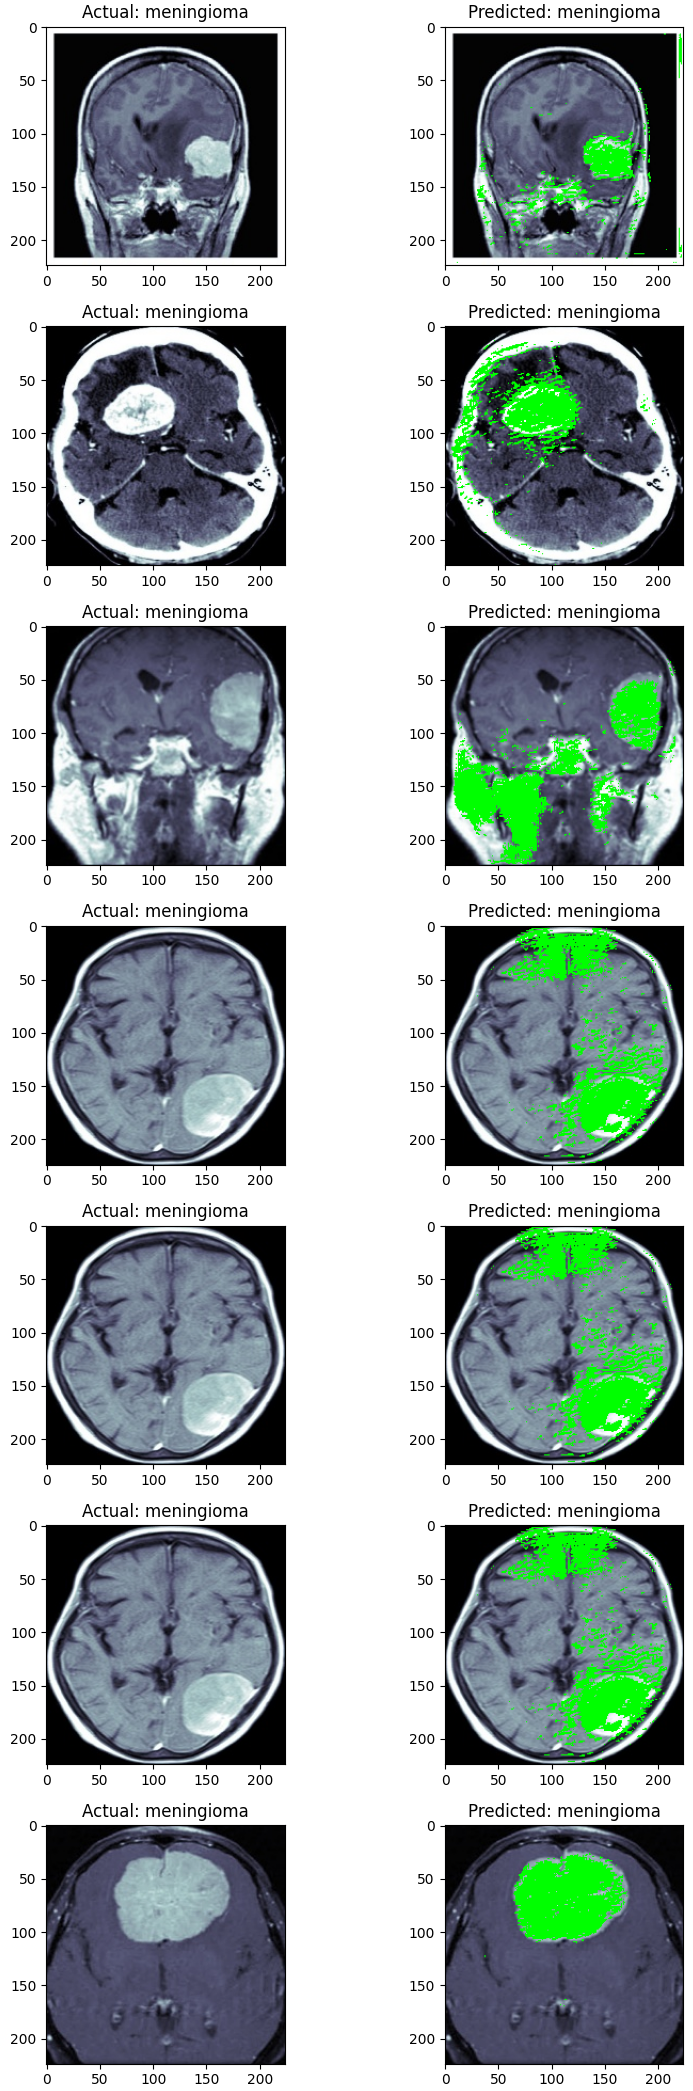
\includegraphics[width=\textwidth]{unet/evaluation/meningioma_3.png}
  \end{subfigure}
  \hfill
  \begin{subfigure}[b]{0.23\textwidth}
    \centering
    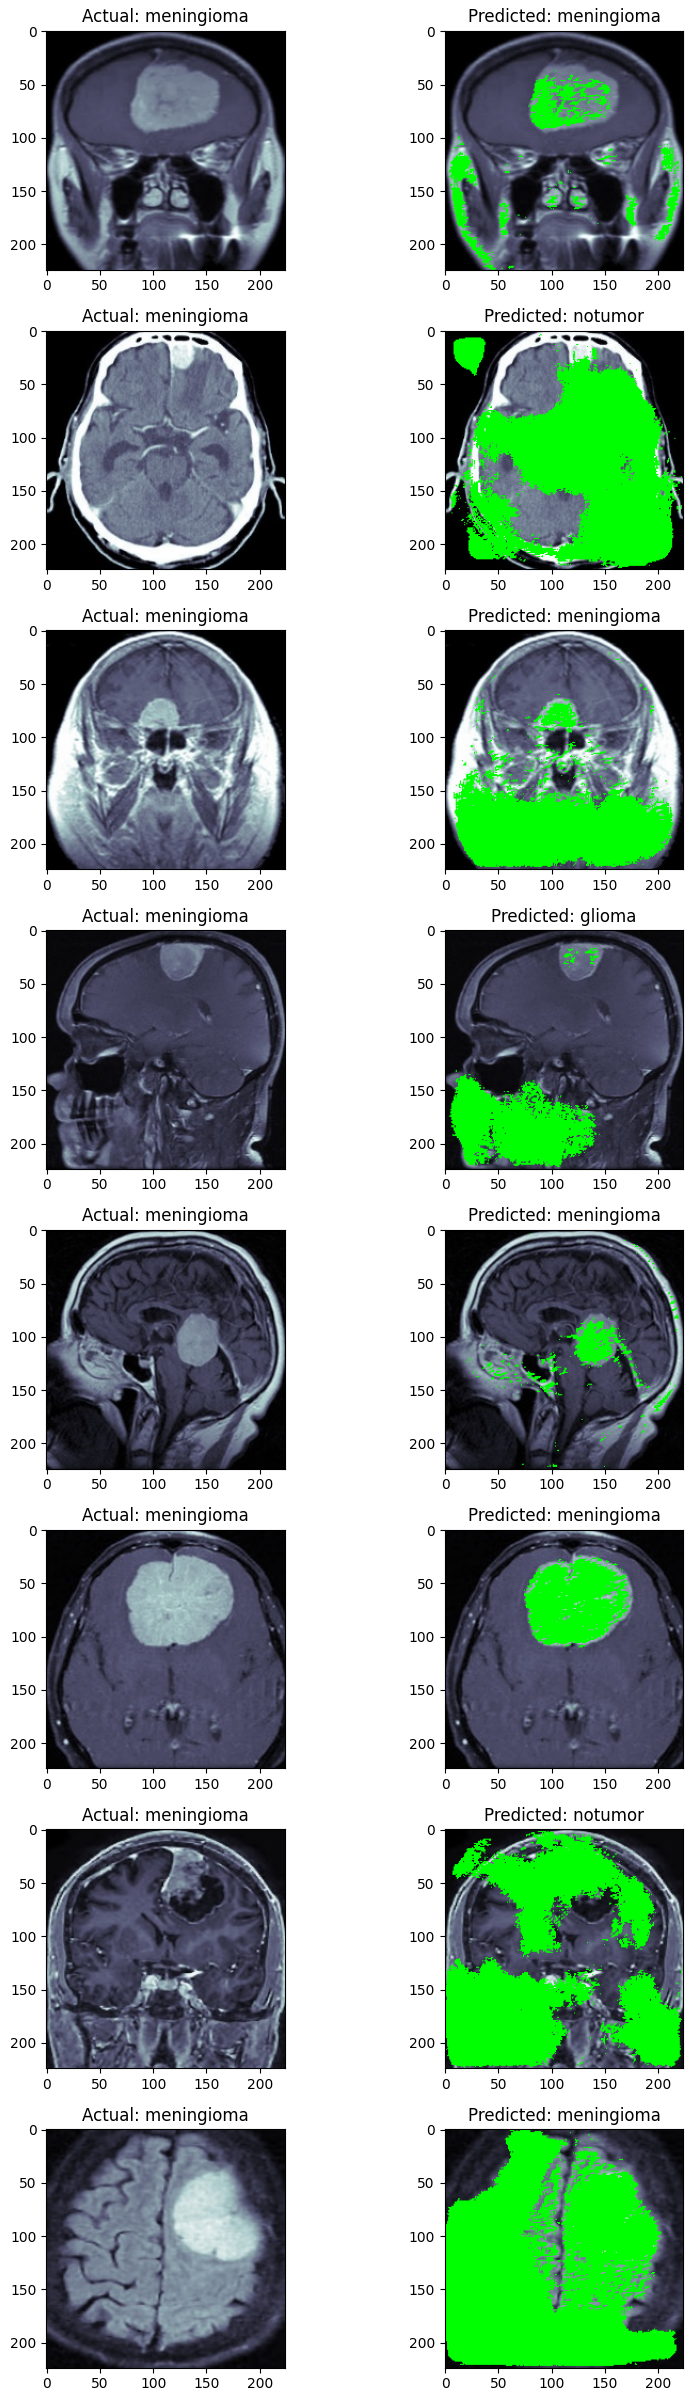
\includegraphics[width=\textwidth]{unet/evaluation/meningioma_4.png}
  \end{subfigure}
  \caption{Additional Segmentation Results for Menigioma}
  \label{fig:additional_malignoma_segmentation}
\end{figure}

Notice that the segmentation results are not perfect, but they are able to capture the general shape of the tumor. Some images that are predicted to not be part of the meningioma are also highlighted, since they are predicted to be part of another tumor.

%\includepdf[
%    %% Include all pages of the PDF
%    pages=-,
%    %% make this page have the usual page style
%    %% (you can change it to plain etc). By default pdfpages
%    %% sets the pagecommand to \pagestyle{empty}
%    pagecommand={\pagestyle{headings}},  
%    %% Add a "section" entry to the ToC with the heading
%    %% "Quilling Shapes" and the label "sec:shapes"
%    %addtotoc={1,section,1,Quilling Shapes,sec:shapes}
%    ]
%%% The pdf file itself
%{unet.pdf}
